\chapter{\toolname{}的实现}

本章介绍了\toolname{}的实现,
介绍了整体架构、谓词生成模块、频谱信息收集模块和怀疑度计算模块等。

\section{整体架构}

章\ref{sec:fl_frame}中已经描述了本文要实现的缺陷定位框架。
这个缺陷定位框架如图\ref{fl_frame1}所示,一共包含三个大的模块:
谓词生成模块,频谱信息收集模块,和怀疑度计算模块。
\begin{figure}[htbp] 
\centering 
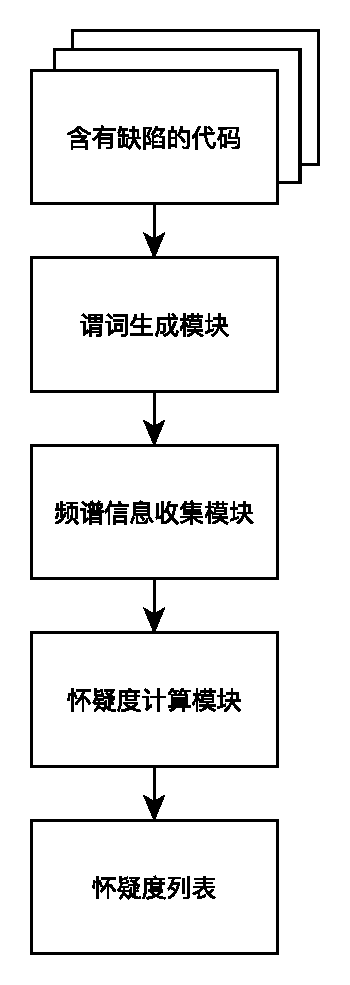
\includegraphics[width=5cm]{figure/frame1} 
\caption{缺陷定位框架模块图} 
\label{fl_frame1}
\end{figure}

谓词生成模块生成预定义的谓词,或者利用机器学习模型预测出谓词。
频谱信息收集模块把生成的谓词插装到缺陷代码,执行测试用例,收集测试用例覆盖谓词真假分支的情况。
最后怀疑度计算模块利用频谱信息,带入公式中计算怀疑度。

具体的流程图如图\ref{fl_frame2}所示。下面将会具体讲述这些步骤的实现。

\begin{figure}[htbp] 
\centering 
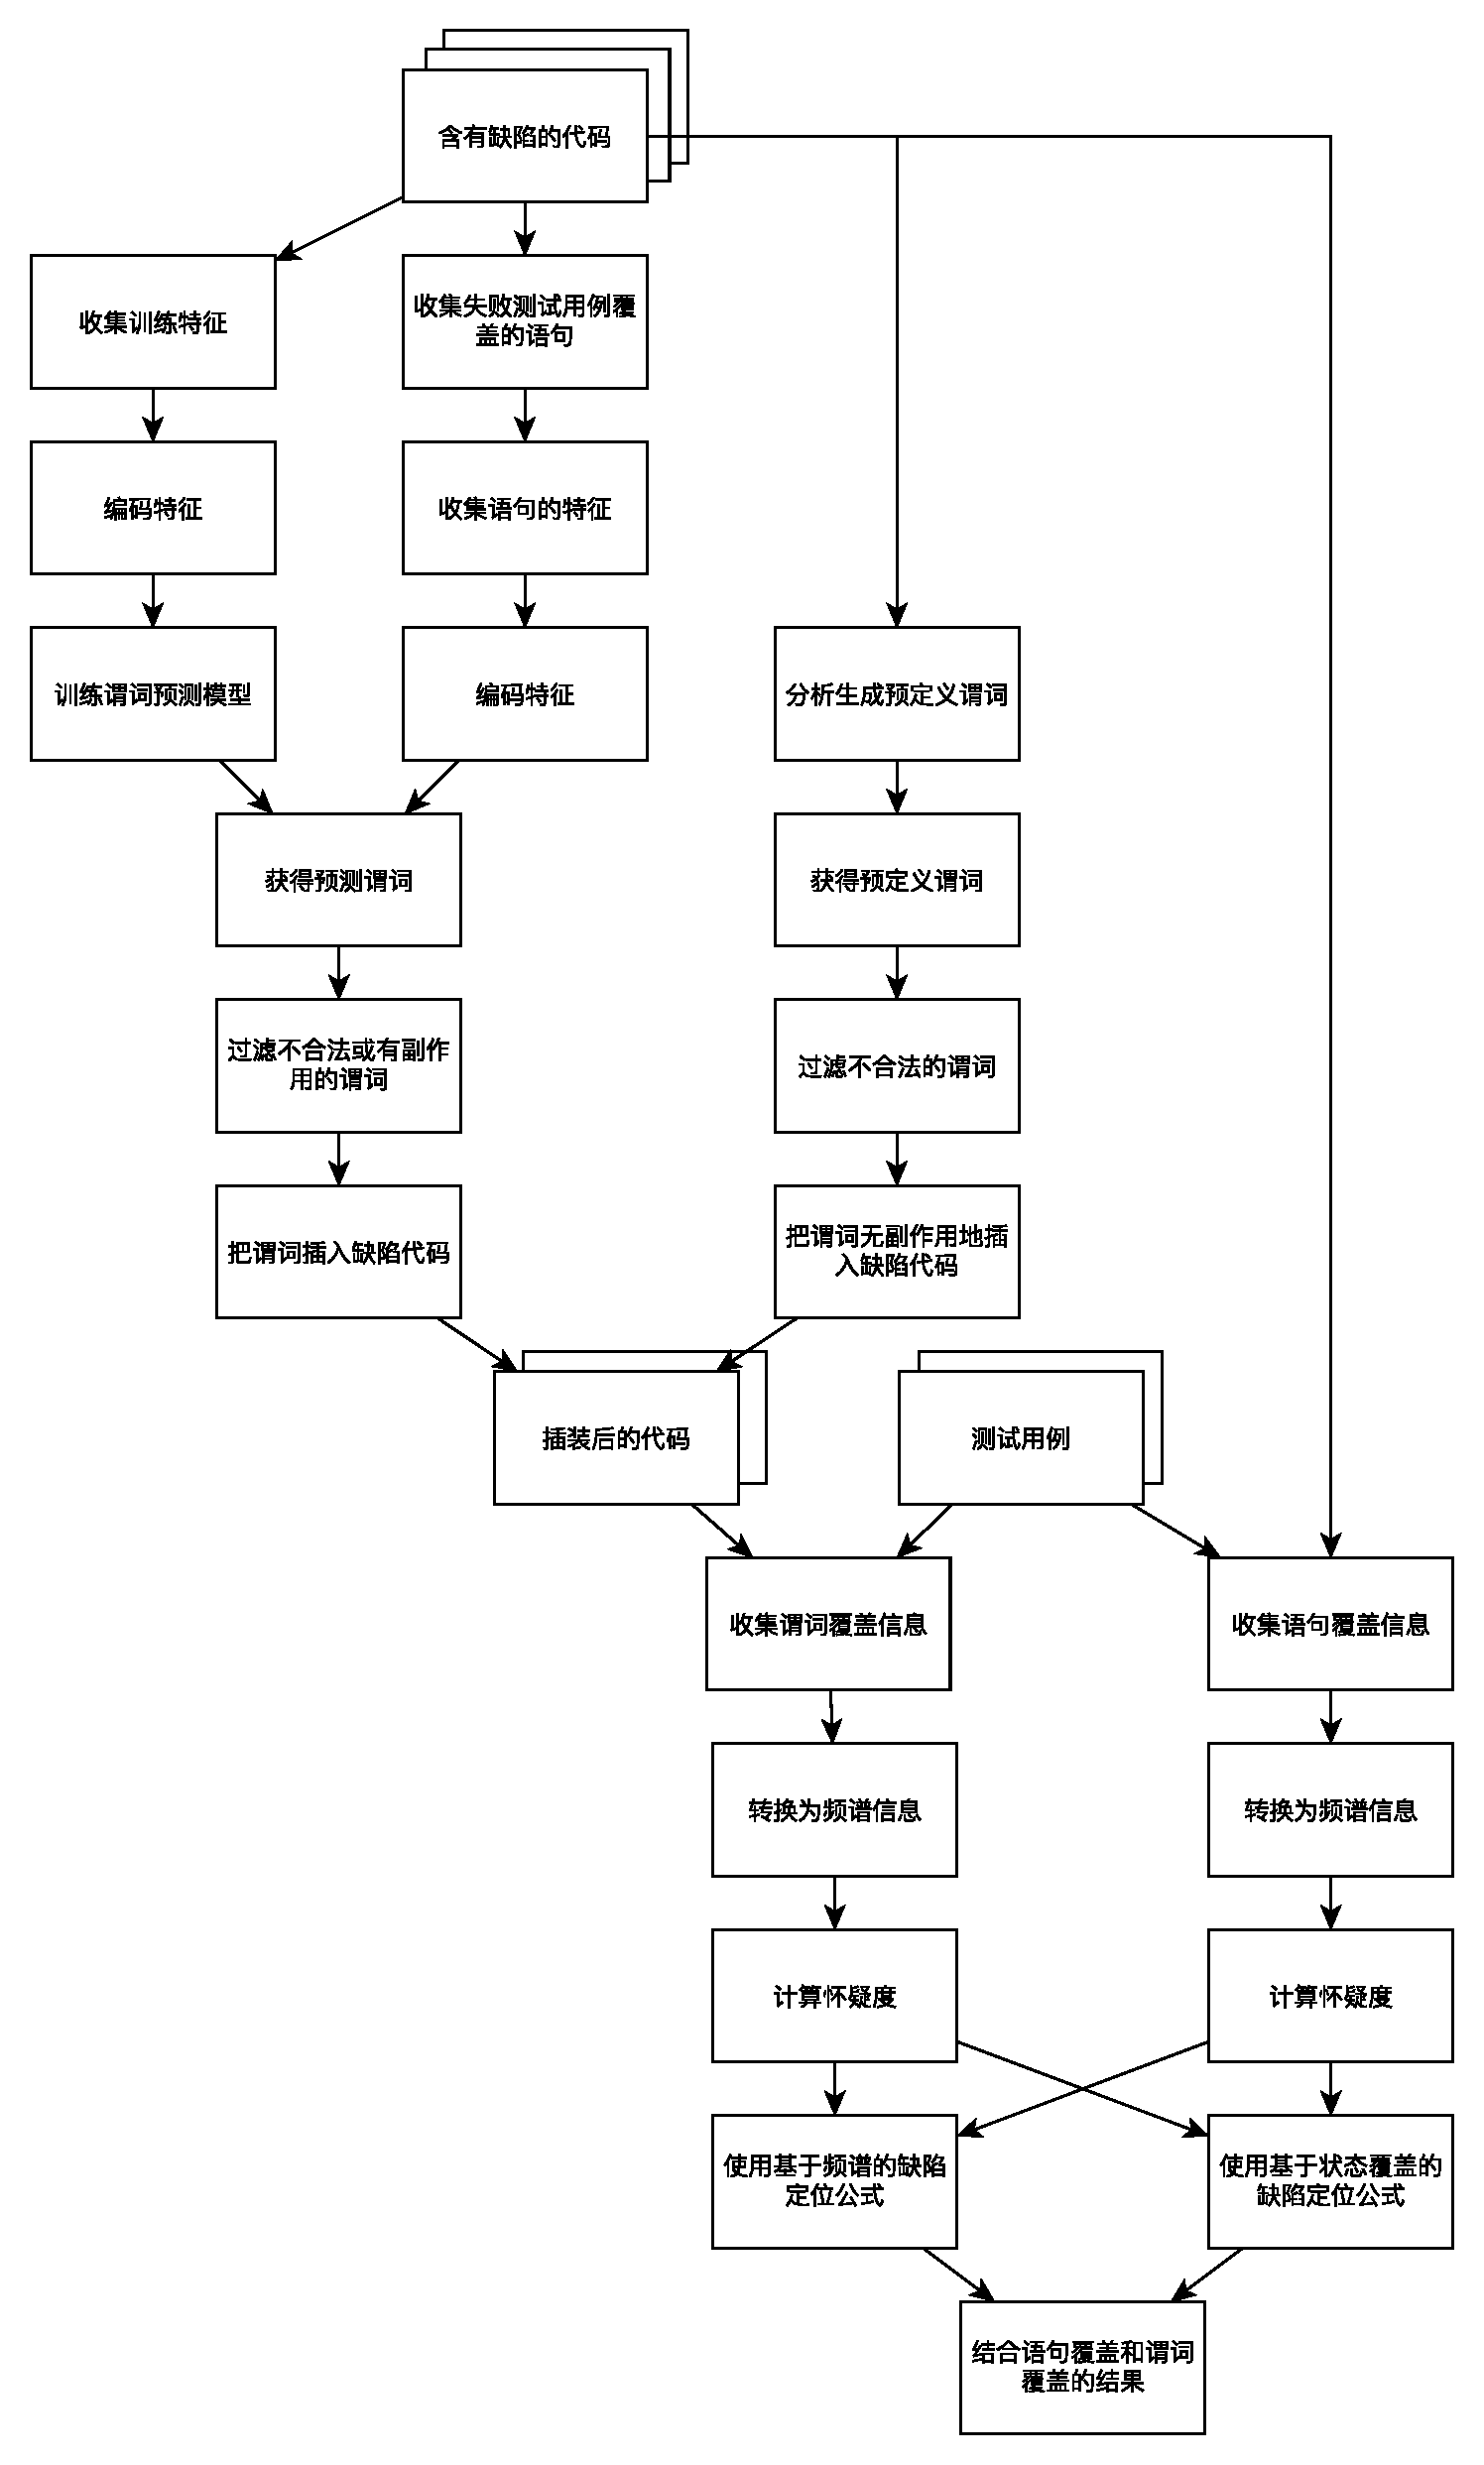
\includegraphics[width=13cm]{figure/frame2} 
\caption{缺陷定位整体流程图}
\label{fl_frame2}
\end{figure}

\section{谓词生成模块}

谓词生成模块负责生成后续会使用的谓词.
谓词生成模块分为两种,一种是生成预测谓词,一种是生成预定义谓词。
生成谓词的语句都是被失败的测试用例覆盖的语句。

\subsection{生成预测谓词模块}
\label{sec:gen_pred_impl}

生成预测谓词使用的是机器学习模型,使用Java和Python实现。
首先,Java代码遍历缺陷代码的抽象语法树,提取表\ref{var_feature}中的特征。
对抽象语法树的处理采用的工具是 eclipse 提供的Java Development Tool\footnote{\url{http://www.eclipse.org/jdt/}},简称JDT。
JDT不仅可以构造给定Java代码的抽象语法树,还可以新建、修改、插入、删除抽象语法树从而新建、修改、插入、删除Java代码。
本章中很多实现都依赖于JDT。
提取的特征被写入到磁盘上的 csv 文件中。
Python程序则读入 csv 文件中的特征,对特征进行编码和训练。

编码阶段,先对变量名、文件名、函数名使用scikit-learn\footnote{\url{http://scikit-learn.org/}}的K-Means聚类,其值转为类编号。
聚类模型等被存储到磁盘。
使用 scikit-learn 的 \mycode{LabelEncoder} 对特征 FileName,MethodName,VarName,VarType,LastAssign,BodyUse
和 OutUse 进行编码,归一化为数字,然后使用 \mycode{OneHotEncoder} 转为独热编码。

训练阶段,特征被放入神经网络或者随机森林中。
神经网络使用的全连接神经网络,用TensorFlow\footnote{\url{https://www.tensorflow.org/}}的 \mycode{DNNClassifier} 实现。
TensorFlow 是一个采用数据流图用于数值计算的开源软件库。
图中的节点表示数学操作,图中的线则表示在节点间相互联系的多维数据数组。
VAR模型和EXPR模型的网络都含有六个隐藏层,每层都是64个节点。这个是小部分实验之后得出的比较适合的值。
网络的输入使用 TensorFlow 的 \mycode{numpy\_input\_fn}。
使用这个函数的好处是,输入不需要在一开始的时候就被存储在内存,
而是在需要的时候才生成一个批(batch)的数据。
每次训练以一个批的数据为一次迭代。
VAR模型和EXPR模型的批尺寸(batch size)都为128。
输入数据会被随机打乱(shuffle)。
一个周期(epoch)就是把全部数据输入神经网络训练一次。
输入数据按照$7:3$的比例分为训练集和验证集。
训练时,会先使用训练集训练\mycode{INIT\_EPOCHS}个周期。
这是因为训练开始时,损失变化较大。
此后每次都再输入一个周期,并收集训练集和验证集在输入这个周期后的新模型上的损失和准确率。
程序会收集最近的\mycode{1}到\mycode{2 * TEST\_EPOCHS}个周期的
训练集和验证集的损失,记为$L(i, j)$。
其中$i$表示是最近的第$i$个周期的损失,$j$为\textit{true}的话表示是训练集的损失,为\textit{false}表示是验证集的损失。
然后分别计算\mycode{1}到\mycode{TEST\_EPOCHS},\mycode{TEST\_EPOCHS + 1}到\mycode{2 * TEST\_EPOCHS}
的训练集总损失值
$$
Loss_1 = \mathrm{Loss}(1, TE, true)
$$
$$
Loss_2 = \mathrm{Loss}(TE + 1, 2 * TE, true)
$$
和验证集的总损失值
$$
Loss_3 = \mathrm{Loss}(1, TE, false)
$$
$$
Loss_4 = \mathrm{Loss}(TE + 1, 2 * TE, false)
$$。
其中\textit{TE}表示\mycode{TEST\_EPOCHS},
$\mathrm{Loss}$定义如下:
$$
\mathrm{Loss}(start, end, j) = \sum_{i=start}^{end}{L(i, j)}
$$。
终止训练的条件为
$$
Loss_1 < Loss_2 \ \mathrm{and} \ Loss_3 > Loss_4
$$。
也就是说当训练集的损失仍在下降,但是验证集的损失却开始上升时,
说明出现了过拟合,停止训练。
实现上会使用四个大小为\mycode{TEST\_EPOCHS}的队列,两个存放训练集损失,两个存放验证集损失。
比如对训练集来说,
一个存放\mycode{1}到\mycode{TEST\_EPOCHS}的数据,称为队列1。
一个存放\mycode{TEST\_EPOCHS + 1}到\mycode{2 * TEST\_EPOCHS}的数据,称为队列2。
每新训练完一个周期,得到当前的损失$l_0$,
再从队列1中弹出一个数据$l_1$,从队列2中弹出一个数据$l_2$。
然后,把$l_0$加入队列1中,并更新$Loss_1$:
$$
Loss_1 = Loss_1 - l_1 + l_0
$$。
把$l_1$加入加入队列2中,并更新$Loss_2$:
$$
Loss_2 = Loss_2 - l_2 + l_1
$$。
训练时会记录当前最小的验证集损失,并会把对应的模型存入磁盘。
训练停止后,最小损失对应的模型成为最终模型。
训练使用 \mycode{DNNClassifier} 的 \mycode{train} 方法,
验证损失和准确率使用 \mycode{evaluate} 方法。
神经网络使用的优化算法是 \mycode{ProximalAdagradOptimizer},
初始学习率设置为0.05,L2正则惩罚系数为0.0001。
随机森林使用 scikit-learn 中的随机森林 \mycode{RandomForestClassfier} 。
训练使用其 \mycode{fit} 方法。
训练好的模型被保存在磁盘中。
神经网络模型直接通过设置 \mycode{model\_dir} 参数保存,
随机森林模型使用 pickle\footnote{\url{https://docs.python.org/3/library/pickle.html}} 保存。

预测阶段,对收集的失败测试用例覆盖的语句进行谓词预测。
首先用Java的JDT提取语句中左值变量的特征,然后写入磁盘上的 csv 文件。
Python程序读入 csv 文件中的特征和编码阶段存储的聚类模型。
同时Python程序也会读入训练时使用的 csv 文件,以获取同样的 \mycode{LabelEncoder} 和 \mycode{OneHotEncoder}。
使用聚类模型将特征的变量名、函数名和文件名划入某个已有的分类。
然后用和训练时一样的 \mycode{LabelEncoder} 和 \mycode{OneHotEncoder} 对特征 FileName,MethodName,VarName,VarType,LastAssign,BodyUse
和 OutUse 进行编码。
最后把预测变量的特征传入训练好的VAR模型和EXPR模型中预测。
神经网络通过 \mycode{predict} 方法预测。
该方法返回预测结果的一个列表。
列表中一个元素对应于一个预测输入,该元素的 \mycode{probabilities} 域表示这个样本属于各个标签的概率,
\mycode{classes} 域表示这个样本的预测标签。
随机森林通过 \mycode{predict\_proba} 方法预测,得到一个矩阵。每行对应一个样本,每列对应这个样本属于某个标签的概率。
VAR模型会输出这个变量出现在谓词中的概率,EXPR模型会对一个样本的概率值排序,取概率最高的200个输出。
最后,将同一个变量其VAR模型的输出$P_{var}$和EXPR模型的输出$P_{pred_i}$相乘,把联合概率大于$0.005$的变量及谓词输出。

验证阶段是在正常的缺陷定位中不存在的阶段。
在测试中被用于测试模型的预测准确性。
在验证阶段,神经网络的输入数据会被使用 scikit-learn 的 \mycode{train\_test\_split} 函数随机分为60\%的训练集,20\%的验证集和20\%的测试集。
然后使用训练集和验证集去训练模型,对得到的模型使用测试集验证其准确率。
随机森林由于会自己划分训练数据,所以把输入数据分为70\%的训练集和30\%的测试集。
准确率使用 scikit-learn 的 \mycode{accuracy\_score} 获得,
而两者的其他评估数值由\mycode{precision\_recall\_fscore\_support}获得。

\subsection{生成预定义谓词模块}

生成预定义谓词使用Java的JDT遍历抽象语法树。

对于一个返回语句,只要其返回值不是空 \mycode{return;},就生成谓词。
对于条件语句 \mycode{if, for, while, do, switch},生成其条件表达式的谓词。
对于赋值语句和变量声明语句,如果其左值是基本数据类型,获取当前行可见的其他同类型变量,生成谓词。

虽然预定义谓词不需要考虑副作用,但是预定义生成的谓词数量往往大于预测谓词的数量。
过滤的时候使用编译过滤速度较慢。
其实预定义谓词并不需要全部过滤。
首先,条件语句的谓词就是其条件表达式和其条件表达式取反,这种谓词肯定是编译正确的,所以不需要过滤。
对于返回语句来说,只要验证 \mycode{v > 0} 是否编译正确就可以知道 \mycode{v < 0} 等谓词是否编译正确。
对于数值对来说,只要验证 \mycode{a > b} 是否编译正确就可以知道 \mycode{a < b} 等谓词是否编译正确。
因此减少了过滤的谓词数量。

\section{频谱信息收集模块} 

频谱信息收集模块主要分为两步,第一步是把谓词插入到代码中,第二步是执行测试用例收集执行信息。
为方便理解,下面将先讲述如何收集执行信息,再讲述如何将谓词插入到代码中。

\subsection{收集频谱信息}

对于谓词$P$和一个测试用例$T_i$,可能需要收集四种信息:
\begin{enumerate}
\item $P$是否被$T_i$观察过(无论是真还是假)。
\item $T_i$中$P$是否至少一次为真。
\item $T_i$中$P$为真的次数。
\item $T_i$中$P$为假的次数。
\end{enumerate}

对于基于频谱的缺陷定位的公式来说,需要第2个信息。
对于统计性调试的公式来说,需要第1、2个信息。
对于SOBER的公式来说,需要第3、4个信息。
所以整体来说谓词的插装有两种形式。
第一种用于基于频谱的缺陷定位公式和统计性调试公式:
\lstset{language=Java}
\begin{lstlisting}
// predicateSignature is a string that uniquely represents the predicate.
SpecLogger.observe(predicateSignature);
if (predicate) {
    SpecLogger.cover(predicateSignature);
}
\end{lstlisting}
\mycode{SpecLogger.observe}记录这个谓词为观察过(信息1),
\mycode{SpecLogger.cover}记录这个谓词为真过(信息2)。
第二种用于SOBER公式:
\lstset{language=Java}
\begin{lstlisting}
// predicateSignature is a string that uniquely represents the predicate.
if (predicate) {
    SpecLogger.coverTrueBranch(predicateSignature);
} else {
    SpecLogger.coverFalseBranch(predicateSignature);
}
\end{lstlisting}
\mycode{coverTrueBranch}记录这个谓词为真的次数(信息3),
\mycode{coverFalseBranch}记录这个谓词为假的次数(信息4)。

这几个\mycode{SpecLogger}的函数可以是把自己内部的某个布尔型的成员变量置为真或假,
也可以是把自己内部的某个整型的成员变量加一。
这个\mycode{SpecLogger}对象在每个测试用例开始的时候重置(使用静态方法变量),并在测试用例结束的时候以某种格式将自己记录的信息输出到文件。
\lstset{language=Java}
\begin{lstlisting}
private void testSomething() {
    SpecLogger.reset();
    SpecLogger.testStatus = true;

    // test ...
    ...

    SpecLogger.dump();
}
\end{lstlisting}
第三行是根据当前测试用例\mycode{testSomething}是通过的测试用例还是失败的测试用例而插装的。
最后\mycode{SpecLogger.dump}把记录的信息输出到文件。
其他程序从这个输出文件中可以构造出频谱信息。

\mycode{SpecLogger.java}会被放入缺陷代码的项目中,成为源码的一部分。
它的方法都被包装成静态函数方便调用。

在代码被插入谓词和记录频谱的语句后,使用测试用例执行代码。
频谱信息会被输出到文件中。
频谱信息分为两类,第一类是SOBER算法的频谱信息。
SOBER算法的每个谓词会对应若干个覆盖信息。
每一条覆盖信息对应一个测试用例的覆盖情况,包含三个数值,分别是谓词为真的次数、谓词为假的次数和当前测试用例是通过还是失败。
第二类是除SOBER以外的公式的频谱信息。
每个谓词对应一条覆盖信息,包含四个数值,分别是谓词真分支被覆盖的失败测试用例个数、谓词真分支被覆盖的通过测试用例个数、谓词(无论真假分支)被覆盖的失败测试用例个数和谓词(无论真假分支)被覆盖的通过测试用例个数。

除了收集谓词的覆盖情况外,还会收集语句的频谱信息,
包括语句被覆盖的失败测试用例个数和被覆盖的通过测试用例个数。

\subsection{不改变程序状态地插入谓词}

预定义的谓词和预测出的谓词都可能有副作用。所以要不改变程序状态地插入谓词。

这两种方法都是使用JDT遍历抽象语法树,然后对函数声明 \mycode{MethodDeclaration} 节点进行一个对其子节点的递归遍历。
这是因为插入谓词涉及到修改语法树,因此对于一个要被修改的节点来说,其父节点是被需要的甚至也是要修改的。

\subsubsection{插入预测谓词}

通过机器学习模型,每个语句可能会关联一组谓词。
但是并不是每个谓词都可以被插入到代码中进行数据收集,因为可能
有不正确的谓词或者有副作用的谓词。
所以需要过滤掉预测出不合法或有副作用的谓词。

过滤包括两步:
\begin{enumerate}
\item 静态分析过滤掉可能不合法的谓词(比如对一个\mycode{int}类型的变量进行下标访问)。
\item 静态分析过滤掉可能有副作用的谓词。
\item 过滤掉不能编译的谓词。
\end{enumerate}

一个预测出来的谓词分为两部分,一个是谓词$P(x)$,一个是变量$v$,最终构成谓词$P(v)$。
一个谓词会被判定为不合法如果它满足以下至少一点:
\begin{itemize}
\item 含有数组访问\mycode{v[i]}且\mycode{v}并不是数组类型。
\item 含有变量访问\mycode{v.a}且\mycode{v}是一个基本数据类型(比如\mycode{int})的变量。
\item 含有变量访问\mycode{a.v}且\mycode{v}不是\mycode{a}的一个域。
% \item \todo{simple name}
\item 含有函数调用\mycode{v.a()}且\mycode{v}是一个基本数据类型变量。
\item 含有函数调用\mycode{f()}且\mycode{f}不属于预定义的合法函数(如\mycode{size},\mycode{length},\mycode{toString},\mycode{contains},\mycode{containsKey},\mycode{Math.abs},\mycode{Double.isInfinite},\mycode{Double.isNaN})。
\item 含有域访问\mycode{v.a}且\mycode{v}是一个基本数据类型的变量。
\item 含有中缀表达式\mycode{a op b}且\mycode{a,b}的类型和运算符\mycode{op}不匹配(比如对非数字类型进行加法)。
\end{itemize}

过滤有副作用的谓词主要是过滤掉以下几种:
\begin{itemize}
\item 含有前缀表达式,且其中运算符为\mycode{++}或\mycode{--}。
\item 含有后缀表达式。
\item 含有赋值语句。
\end{itemize}

最后单独地插入每一条谓词,过滤掉不能顺利编译的。
在没有判定谓词是否合法的时候,也可以通过编译来排除不合法的谓词。
但是由于谓词数量较多,通过预处理去掉部分肯定不对的谓词可以加速整个流程。

这样,对于一个语句$s$,我们可以得到一组合法无副作用的谓词${P_1,P_2...}$,取预测概率最大的前五个作为该语句的谓词。
我们还可以再加入取反的谓词${!P_1, !P_2, ...}$。

然后就是将收集谓词频谱信息的代码插入到语句前或后。
语句前后都插入的有\mycode{whi le,for,do},
插入在语句后面的有赋值语句,
插入在语句前的有\mycode{if,switch}等其他所有语句。

\subsubsection{插入预定义谓词}

预定义的谓词也可能有副作用,比如赋值语句\mycode{a[b++] = c}的谓词\mycode{a[b++] > d},
如果使用此前的插装方法,则插入\mycode{if (a[b++] > d)}这样的语句会产生副作用。
但是如果使用中间变量,则上述代码可以重写为:
\lstset{language=Java}
\begin{lstlisting}
temp = c;
a[b++] = temp;
if (temp > d) {
    ...
}
\end{lstlisting}
所以预定义谓词的三种情况,分支、返回、数值对,都可以使用中间变量这样的方式来插入谓词,从而避免了副作用的情况。

由于分支对应多种情况,使用中间变量会比较复杂。
分支的谓词是分支中含有的条件表达式。
\mycode{Do}中的条件表达式的值每次循环都会更新,再考虑上\mycode{continue}这样的语句,
会让条件表达式的更新逻辑非常复杂。
为了简单地插入谓词,并且由于条件表达式的类型都是布尔型,使用一个函数\mycode{logConditionCoverage}替换条件表达式。
原代码为:
\lstset{language=Java}
\begin{lstlisting}
// example.java:
while(!iter.isEmpty()) {
	...
}
\end{lstlisting}
插装了收集谓词频谱信息的语句后,代码被修改为:
\lstset{language=Java}
\begin{lstlisting}
// example.java
while(SpecLogger.logConditionCoverage(!iter.isEmpty(), "!iter.isEmpty()", "!(!iter.isEmpty())") {
	...
}

// SpecLogger.java
public static boolean logConditionCoverage(boolean condition, String trueLogInfo, String falseLogInfo) {
	observe(trueLogInfo);
	observe(falseLogInfo);
	if (condition) {
		cover(trueLogInfo);
	} else {
		cover(falseLogInfo);
	}
	return condition;
}
\end{lstlisting}
这里同时记录了假分支的覆盖情况。这样做有两个目的:
\begin{itemize}
\item 统计性调试中预定义的分支型谓词有条件表达式取反。
\item 和预测谓词加入了谓词取反的情况保持一致。
\end{itemize}

无副作用地插装时可能会涉及到新建变量、修改原有语句等。
因为无副作用的插入方法会新建一个中间变量,然后用这个中间变量替换原有变量的位置。
比如,为了在 \mycode{return a.increase();} 处插入谓词 \mycode{a.increase() > 0},
首先是使用 \mycode{VariableDeclaratio- nFragment} 新建一个变量,这个变量的变量名组成为
\mycode{"automatic\_" + lineNumber + "\_" + varCount}。
其中 \mycode{lineNumber} 是行号, \mycode{varCount} 是一个递增的新变量计数。
然后把这个 \mycode{VariableDeclarationFragment} 放入更高一层的 \mycode{VarableDeclarationExpression} ,
得到 \mycode{int automatic\_11\_2}。
再将其放入 \mycode{Assignment},得到 \mycode{int automatic\_11\_2 = a.increase();}。
把原本的返回语句改为 \mycode{return automatic\_11\_2;}。
然后谓词也要修改,
原本要插入的谓词是 \mycode{a.increase() > 0},
现在要插入的谓词应该是 \mycode{automatic\_11\_2 > 0}。

\section{怀疑度计算模块}

怀疑度计算模块根据频谱信息的不同也分为两种。
一种是SOBER算法的怀疑度计算,一种是其他算法的怀疑度计算。
在实现上,SOBER算法继承一个父类,其他算法继承另一个父类。
子类需要实现两个函数,一个是 \mycode{getName} 返回算法名,
一个是 \mycode{getScore} 返回怀疑度。
父类负责从磁盘读取执行信息并处理为频谱信息,计算并结合语句的怀疑度和谓词怀疑度,根据怀疑度对语句进行排序,最后输出到磁盘。
% 具体的结合方式根据会在

在一条语句的多个谓词中,选择怀疑度最高的作为这个语句的最终谓词怀疑度。结合方式有\textsc{MaxPred}和\textsc{LinPred}。


